Caught up part of Deep-Vision workshop. I was a little bit confused on overwhelming tutorials and workshops. I also spent a lot of time trying to find the correct room. So first day's note was not really good. Please feel free to contact me and add some notes.

\subsection{Workshop: Deep-Vision}
\subsubsection{Topic: AI on Medicine, Speaker: Serena Yeung}
Arrived at the end of the talk on this topic. She talked about Learning from few labeled training examples \\
\textbf{Learning to learn from noisy web videos (CVPR2017)}\newline
{\bf Idea:} Proposed a Reinforcement learning-based method for learning data labeling form noisy web videos. Result is able to learn domain-specific knowledge, and label data for new classes while avoiding semantic drift.\\
\\
\begin{figure}[]
    \centering
    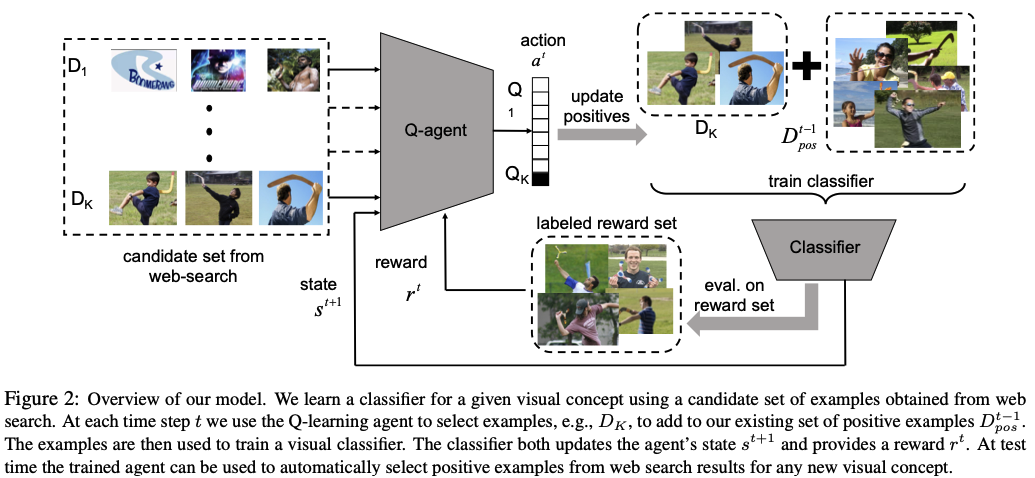
\includegraphics[width=1\textwidth]{images/Image4.png}
    \label{fig:Conf_D1_1}
\end{figure}\\
{\bf Terminology:} \textit{candidate set:} noisy search result. \textit{reword set:} a set of examples annotated with the presence or absence of the target class.\\
\\
\textbf{Temporal Modular Networks for Retrieving Complex Compositional Activities in Videos (ECCV2018)}\\
\\
\textbf{Neural Graph Matching Networks for Fewshot 3D Action Recognition (ECCV2018)}\\
\\
Talked about Towards full realization of an AI-assisted hospital: Integration of multimodal data sources. \\
Talked about Jointly Learning Energy Expenditures and Activities using Egocentric Multimodal Signals (CVPR 2017) \\
Will add a short paper summary here... \\

\subsubsection{Topic: Video Re-Id, Speaker: Prof. Dr. Laura Leal-Taixé}
Tractor++ (reId+CMC)\\
CMC = motion camera model
\subsubsection{Topic: Video Super-resolution, Speaker: Prof. Dr. Laura Leal-Taixé}
Designed new Temporal Loss to improve video SR performance. Great results.
\subsubsection{Topic: Google Brain Pierre Sermanet: Self-Supervision and Play}
-Label Free\\
-Time-Contrastive Networks (TCN)\\
-Object-contrastive Networks\\

